\documentclass[12pt]{article}
\usepackage{graphicx}
\def\figdir{mfigs}

\begin{document}
\title{Report on using the NERSC Edison computer}

\author{Bj{\"o}rn Sj{\"o}green and N. Anders Petersson}

\maketitle

\section{Introduction}

We used the time allocated on Edison to test out a newly developed material 
inversion capability, built on the linear elastic and anelastic wave propagation code, SW4 \cite{SW4}. 
The material inversion was done by full wave form inversion in the time domain. 
The inversion algorithm minimizes the misfit between computed and observed time 
series (seismograms) at a few locations on the surface of the computational domain. 
A gradient based minimization algorithm was used, where each evaluation of the gradient required
solution of the elastic wave equation and its adjoint.

Our usage consisted mainly in running the code, we did not perform any code development on Edison.

\section{Experience of running on Edison}
We do not have experience of running on Vulcan or Sequoia. SW4 was developed on Cab at LC and, hence, we 
can only compare Edison with Cab.
Our experience is with the Phase 1 of the Edison machine. The hardware on Edison is similar to the hardware on 
Cab. Both machines have two 8 core Intel Xenon processors per node, giving 16 cores per node. Edison had larger
memory, 64 Gbyte/node vs.~32 Gbyte/node for Cab.

The software environments on Cab and Edison were similar. We had no difficulty in buliding SW4 on Edison 
using the default version of the GNU compilers and the MPICH2 MPI library. SW4 in its basic version 
does not need other external libraries. Edison uses a different queue system than Cab (Torque vs.~Moab), 
but once learning the different commands, submitting jobs on Edison worked similarly to Cab, and without problems.

The code made extensive use of the parallel file system on Edison, since computing the gradient of the misfit, needed
in the material inversion, involves combined forward and backward solves, where the time history of all data 
on the far-field boundaries are saved to disk during the forward solve (there is too much data to keep in
memory), and read back in when performing the backward solve. We found that this worked without 
difficulties, although the time to solution can vary considerably depending on the load of the file system.
However, the sensitivity to the file system load on Edison was not worse than at LC.

The performance of the code was similar on Edison and Cab. We did not make any systematic performance study. 
One saved data point is for one problem size that were run on 1024 cores on both machines. The wall clock
times was about 37 seconds per iteration on Edison and 41 seconds per iteration on Cab.

Overall, we are very satisfied with Edison. Everything worked as expected, and in a very similar way to
Cab, the computer we used at LC.

\section{Accomplishments}
The material inversion capability was tested out on a few synthetic examples. The purpose was both to 
validate the code, and to gain experience on the behavior of the algorithm when varying some input
parameters. In particular, we made extensive experimentation with different ways to scale the unknown
variables in order to find a scaling strategy that gives rapid convergence to the minimum. 

An example is shown in Fig.~\ref{fig:1} below, where a problem on a domain of 
size 35000$\times$35000$\times$17000 is solved. A traction free boundary condition is imposed
on the surface $z=0$. The other five sides are far-field boundaries. Waves are generated by a single 
moment source at depth $z_s=2000$.
The unknowns are the three fields, density, and the Lam\'e parameters $\mu$, and $\lambda$. 
Synthetic seismograms were produced at 25 locations on the surface $z=0$, by solving the forward problem 
with given, non-constant, density, $\mu$, and $\lambda$. The minimization algorithms starts from a constant
material and minimizes the misfit between the computed and synthetic seismograms with respect to the 
three material fields.
Figure~\ref{fig:1} shows how the Lam\'e parameter $\lambda$ on the plane $z=1000$ converges to the 'exact' 
minimum as the iterations proceed. 

The convergence history in Fig.~\ref{fig:2} shows that around 200 iterations were required to bring down 
the misfit (red) to its minimum and the norm of the gradient close to zero (blue). For this computation, with
400 iterations, the elastic wave equation was solved 1600 times, since each iteration in the optimization algorithm 
requires four solves of the elastic wave equation.  Clearly, a powerful computer is required for this type of 
computation. 

The early user program program on Edison helped us to speed up the development of the material inversion 
capability. We are very grateful for having been given the oportunity to run on Edison.

\begin{figure}
\begin{center}
\includegraphics[width=0.33\textwidth]{\figdir/la-it1.png}\hfil
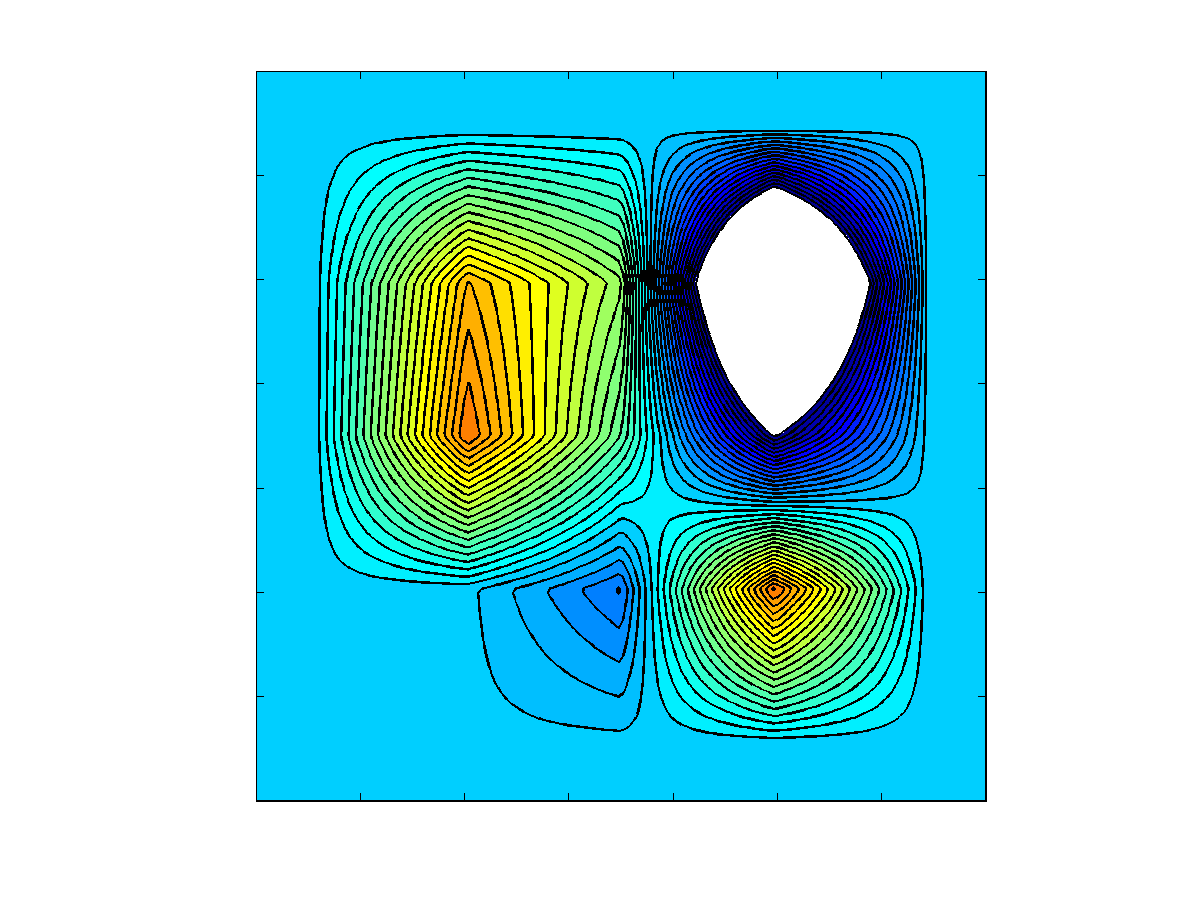
\includegraphics[width=0.33\textwidth]{\figdir/la-it10.png}\hfil
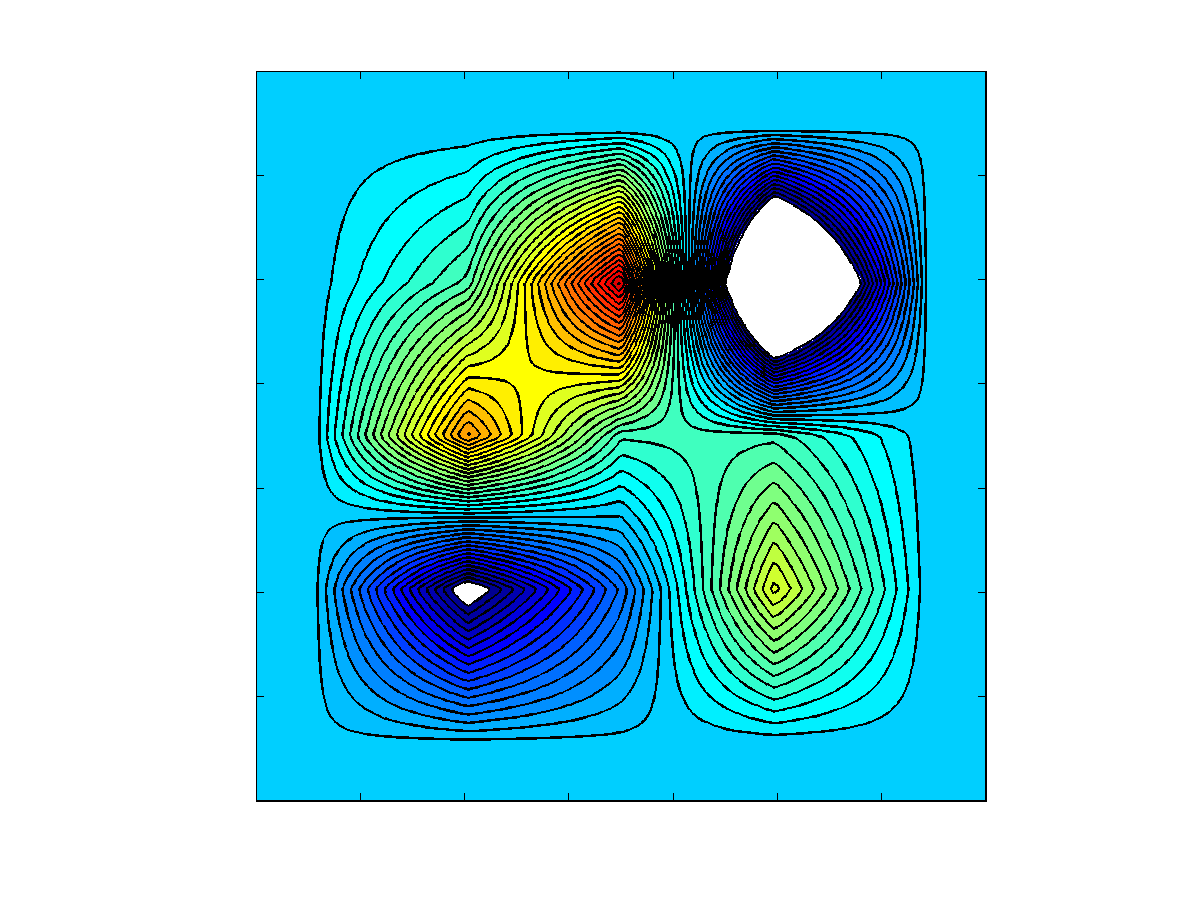
\includegraphics[width=0.33\textwidth]{\figdir/la-it20.png} \\
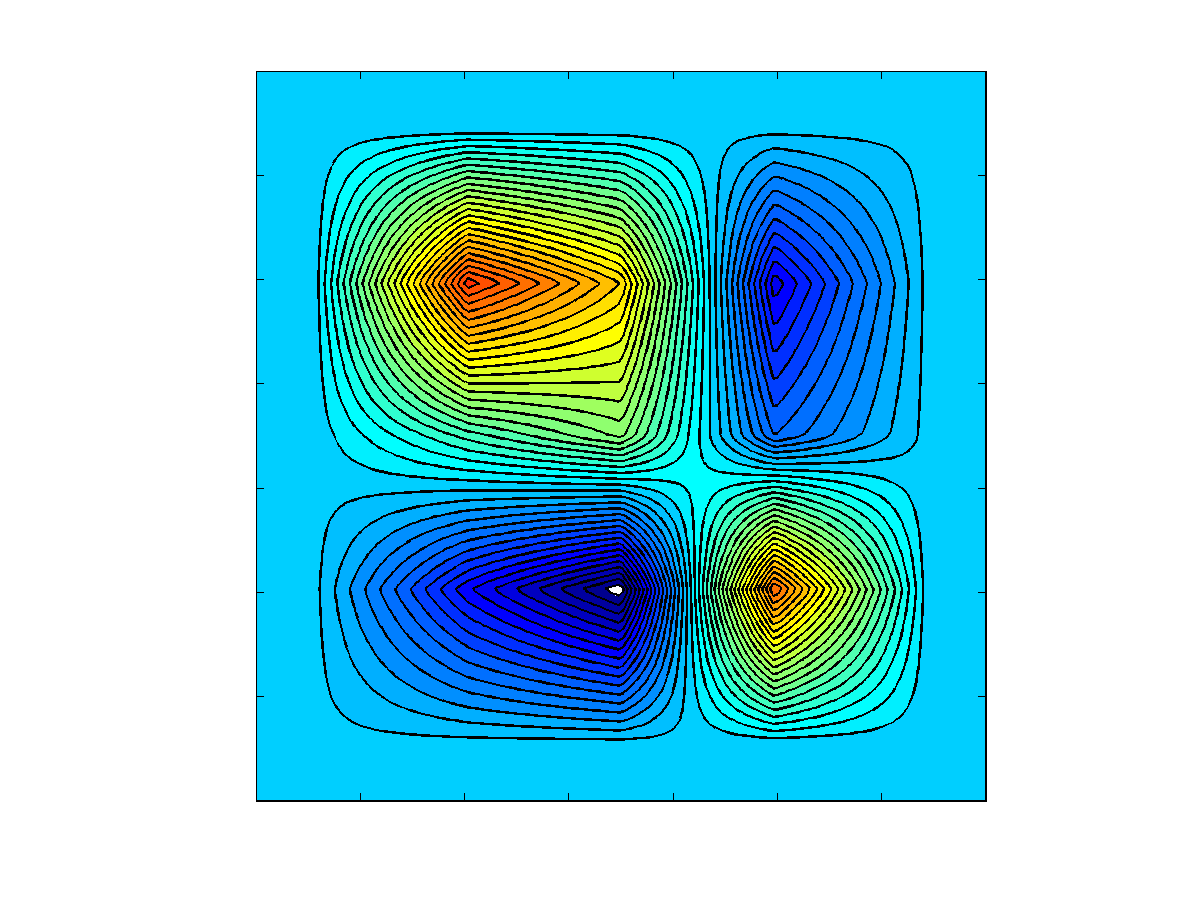
\includegraphics[width=0.33\textwidth]{\figdir/la-it30.png}\hfil
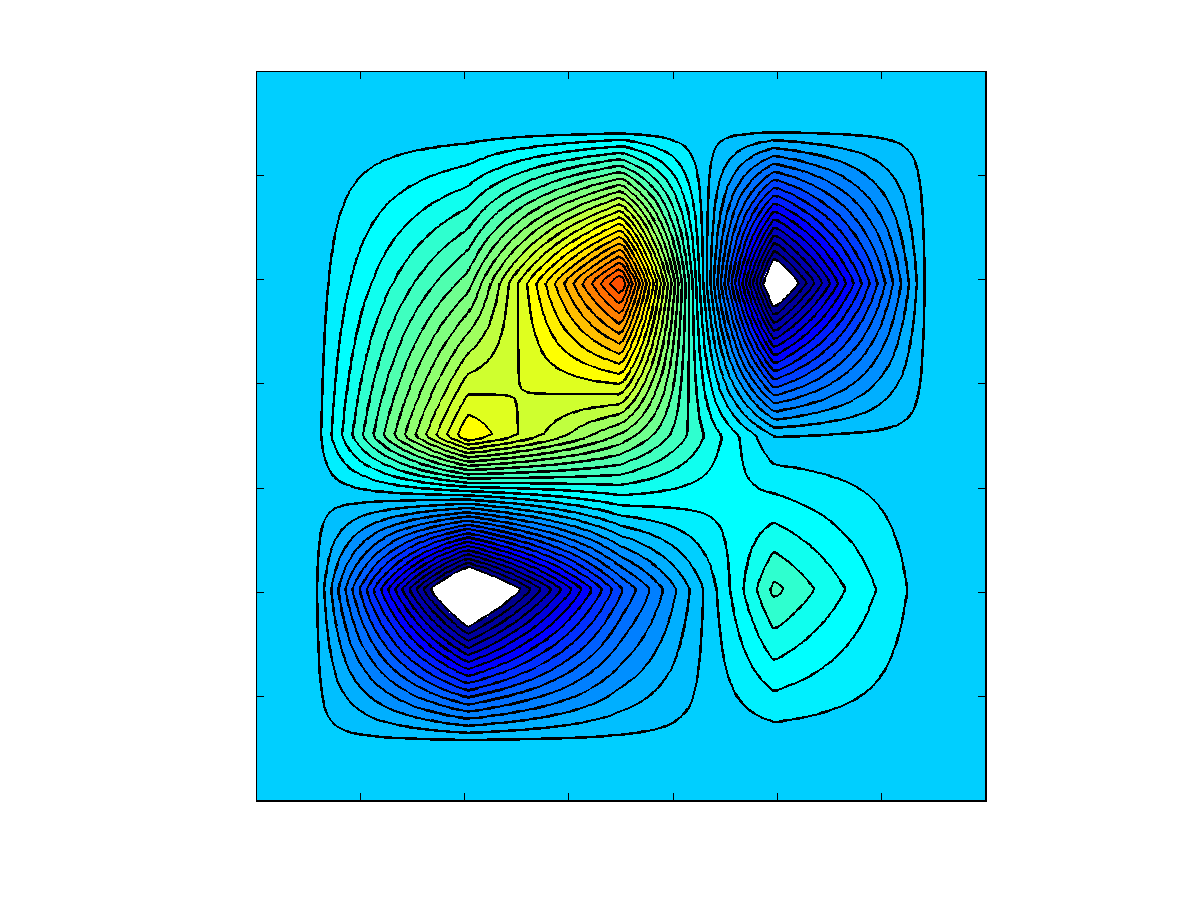
\includegraphics[width=0.33\textwidth]{\figdir/la-it40.png}\hfil
\includegraphics[width=0.33\textwidth]{\figdir/la-it50.png} \\
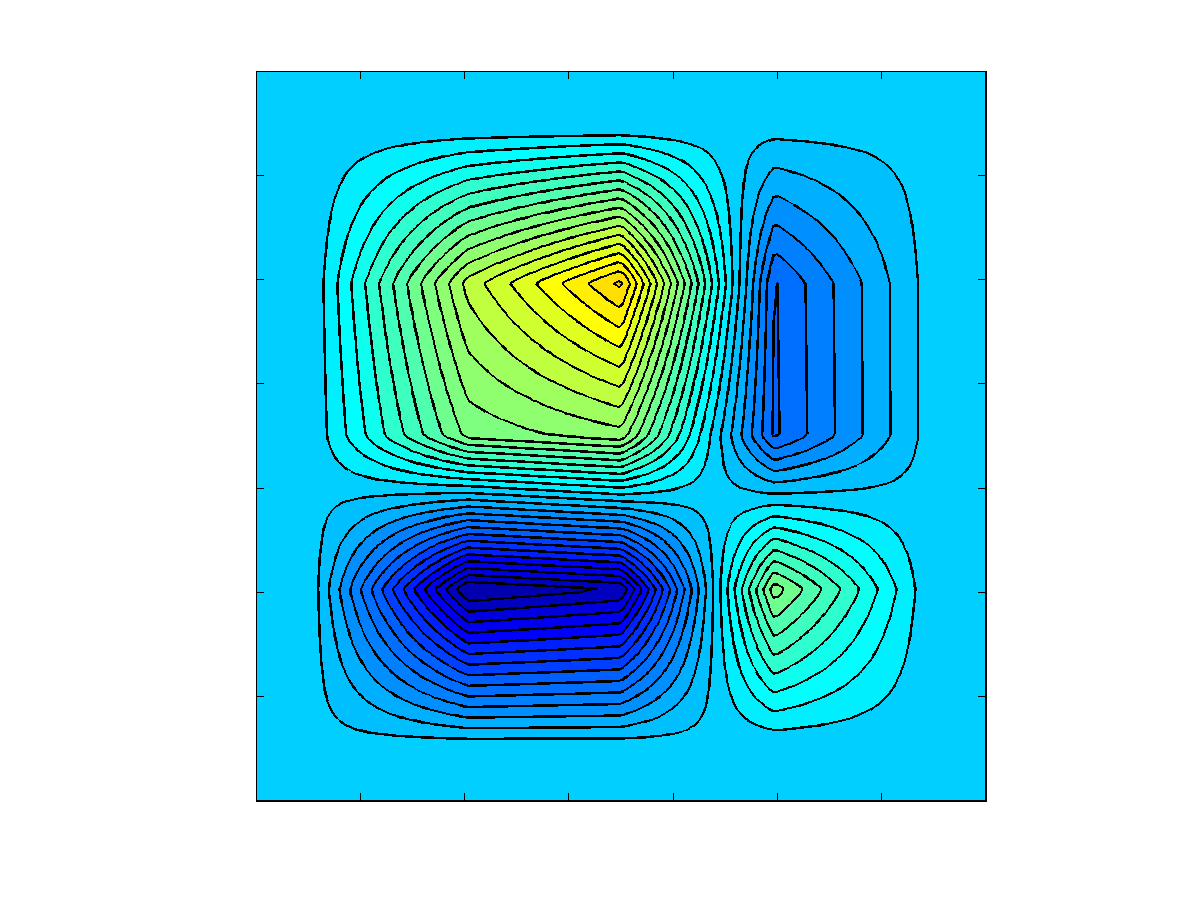
\includegraphics[width=0.33\textwidth]{\figdir/la-it60.png}\hfil
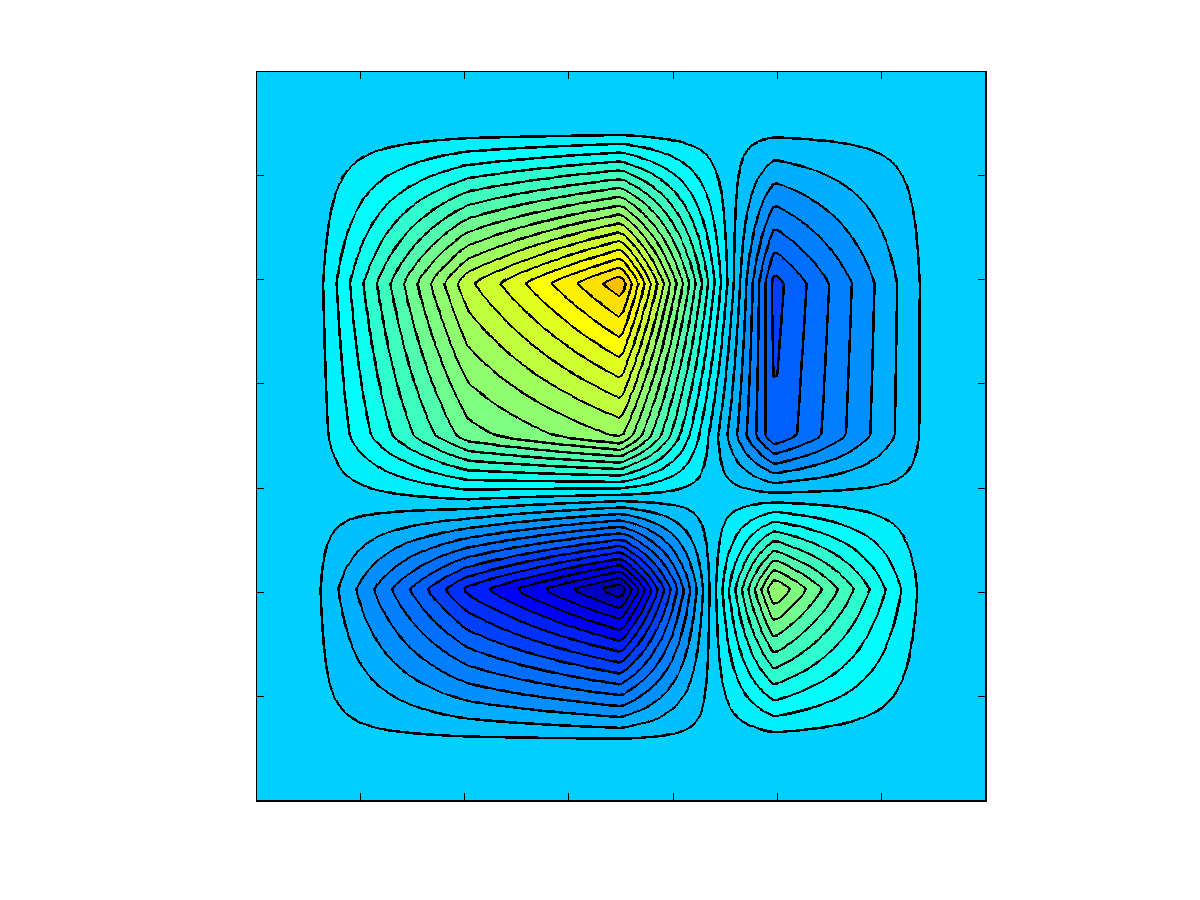
\includegraphics[width=0.33\textwidth]{\figdir/la-it70.png}\hfil
\includegraphics[width=0.33\textwidth]{\figdir/la-it80.png} \\
\caption{Lam\'e parameter $\lambda$ on the plane $z=1000$ after 1, 10, 20, 30, 40, 50, 60, 70, and 80 iterations
with the L-BFGS method.}
\label{fig:1}
\end{center}
\end{figure}

\begin{figure}
\begin{center}
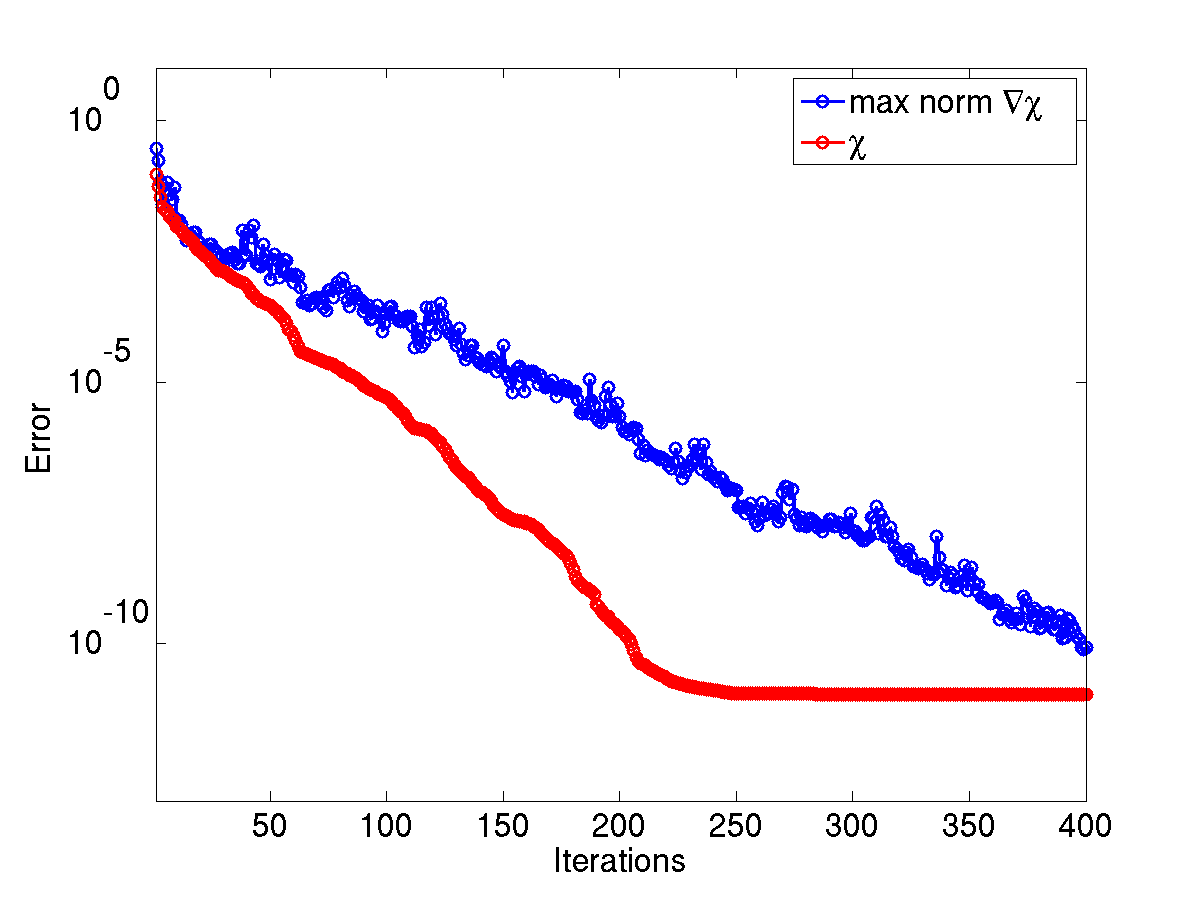
\includegraphics[width=0.7\textwidth]{\figdir/conv-run6.png}\hfil
\caption{Convergence of misfit (red) and maximum norm of the gradient of the misfit (blue) for 
the computation shown in Fig.~\ref{fig:1}.}
\label{fig:2}
\end{center}
\end{figure}

\begin{thebibliography}{99}
\bibitem{SW4} N.A.Petersson and B.Sj\"ogreen, ``User's guide to SW4 version 1.0'', Lawrence Livermore National
Laboratory, LLNL-SM-642292.
\end{thebibliography}

\end{document}